\documentclass{beamer}
\usetheme{Madrid}

\usepackage{amsmath, amssymb, amsthm}
\usepackage{graphicx}
\usepackage{gensymb}
\usepackage[utf8]{inputenc}
\usepackage{hyperref}
\usepackage{tikz}


\title{9.3.3 Matgeo}
\author{AI25BTECH11012 - Garige Unnathi}
\date{}

\begin{document}

\frame{\titlepage}

% Question frame
\begin{frame}
\frametitle{Question}
Find the area enclosed by the parabola 4y = 3$x^2$ and the line 2y = 3x + 12.\\
\end{frame}


% Solution steps
\begin{frame}
\frametitle{Solution}
The points of intersection of the line :

\begin{align}
  L : \textbf{x} = \textbf{h} + \kappa\textbf{m}
\end{align}

with the conic  is given by 
\begin{align}
   \textbf{x}_i = \textbf{h} + \kappa_i\textbf{m}
\end{align}
\end{frame}


\begin{frame}
\frametitle{Solution}
where :

\begin{align}
 g(\textbf{x}) = \textbf{x}^{T}\textbf{V}\textbf{x} + 2\textbf{u}^{T}\textbf{x} + f \\
\kappa_i = \frac{1}
{\textbf{m}^{T}\textbf{V}\textbf{m}}(-\textbf{m}^{T}(\textbf{V}\textbf{h} + \textbf{u}) \pm \sqrt{[\textbf{m}^{T}(\textbf{V}\textbf{h}+\textbf{u})]^{2} - g(\textbf{h})(\textbf{m}^{T}\textbf{V}\textbf{m})})
\end{align}
\end{frame}


\begin{frame}
\frametitle{Solution}
For the parabola 3$x^2$ - 4y = 0
\begin{align}
   \textbf{V} = \begin{bmatrix}3 & 0\\0& 0\end{bmatrix}\\
   \textbf{u} = \begin{bmatrix}0\\-2\end{bmatrix}
\end{align}
For the line  2y = 3x + 12.
\begin{align}
  \textbf{X} = \begin{bmatrix}0\\6\end{bmatrix} + \kappa\begin{bmatrix}0 \\ \frac{3}{2}\end{bmatrix}\\
  \textbf{h} = \begin{bmatrix}0\\6\end{bmatrix}\\
  \textbf{m} = \begin{bmatrix}0 \\ \frac{3}{2}\end{bmatrix}
\end{align}
\end{frame}

\begin{frame}
\frametitle{Solution}
Substituting and solving we get :
\begin{align}
 \kappa = \begin{bmatrix}2 \\ -1\end{bmatrix}
\end{align}
so the points of intersection after solving using the equation 0.2 are :
\begin{align}
    \textbf{X} = \begin{bmatrix}4 \\ 12\end{bmatrix} \quad and \quad \begin{bmatrix}-2\\3\end{bmatrix}
\end{align}
Calculating the area  :
\begin{align}
    \int_{-2}^{4} \frac{3}{2}x + 6 - \frac{3}{4}x^2\,dx = 27 
\end{align}
\end{frame}


% Graphical representation
\begin{frame}

\frametitle{Graphical Representation}
\begin{center}
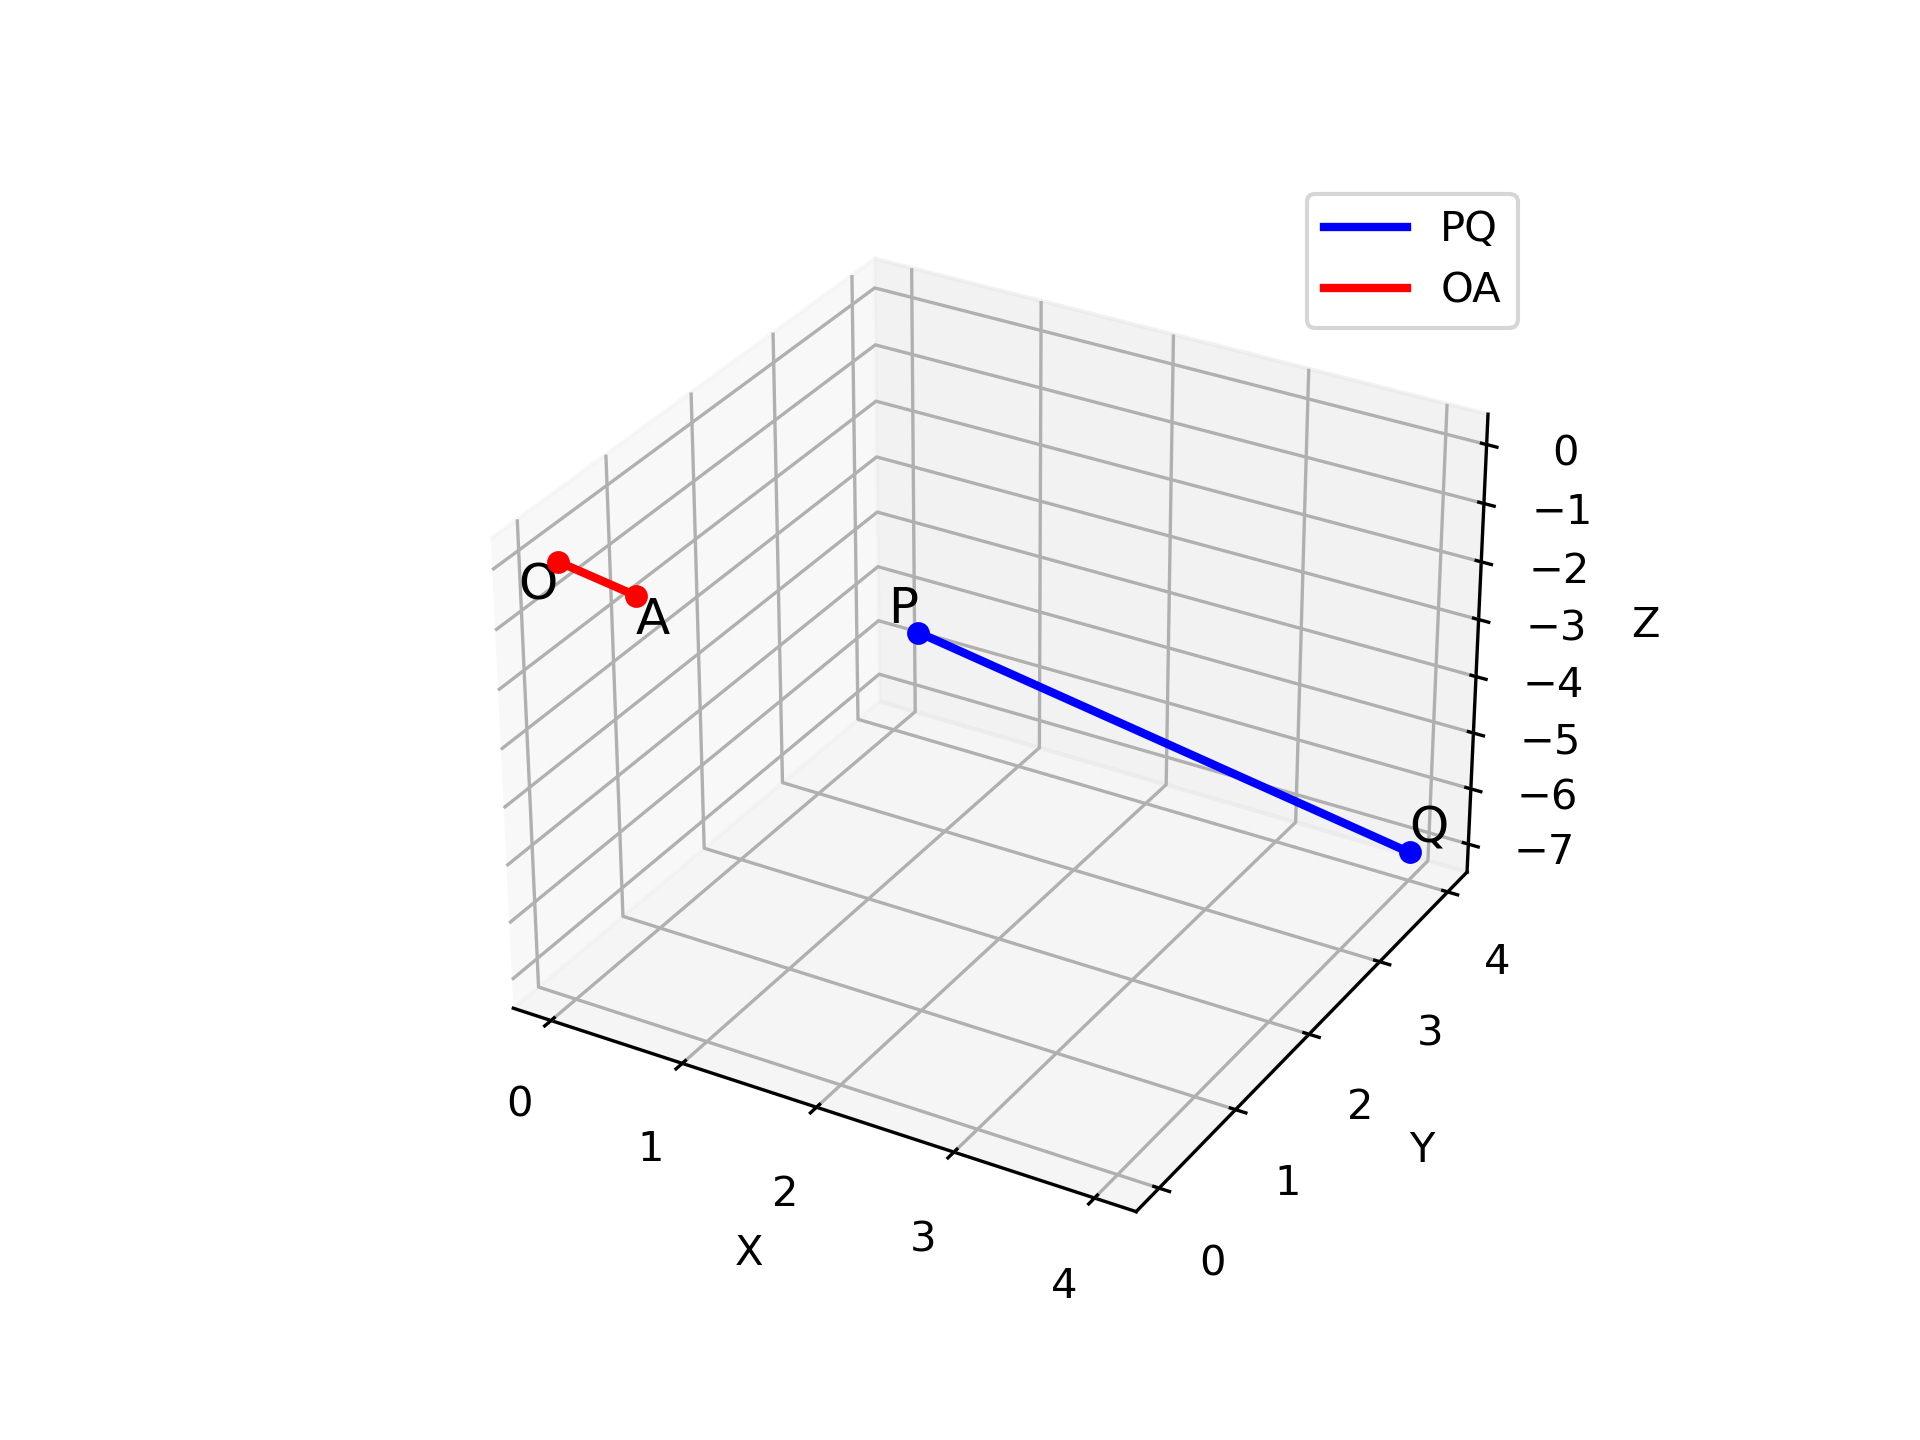
\includegraphics[width=0.6\linewidth]{/Users/unnathi/Documents/ee1030-2025/ai25btech11012/matgeo/9.3.3/figs/fig.png}
\end{center}
\end{frame}

\end{document}
